\documentclass[a4paper,12pt]{article}
\usepackage[utf8]{inputenc}
\usepackage[english]{babel}
\usepackage{graphicx}
\usepackage{geometry}
\usepackage{listings}
\usepackage{xcolor}
\usepackage{tikz}
\usetikzlibrary{shapes, arrows, positioning, calc}

\geometry{top=2cm, bottom=2cm, left=2.5cm, right=2.5cm}
\definecolor{codegreen}{rgb}{0,0.6,0}
\lstdefinestyle{mystyle}{
    backgroundcolor=\color{white},   
    commentstyle=\color{codegreen},
    keywordstyle=\color{blue},
    basicstyle=\ttfamily\footnotesize,
    breakatwhitespace=false,         
    breaklines=true,                 
    captionpos=b,                    
    keepspaces=true,              
    numbers=left,                    
    numbersep=5pt,                  
    showspaces=false,                
    showstringspaces=false,
    showtabs=false,                  
    tabsize=2,
    frame=single
}
\lstset{style=mystyle}

\title{\textbf{Practical Work 4: Word Count using MapReduce}}
\author{Group ID: 16}
\date{\today}

\begin{document}

\maketitle

\section{Introduction}
This report presents the implementation of the classic \textbf{Word Count} problem using the MapReduce programming model. The goal is to count the frequency of each word in a given text dataset by distributing the task across Mapper and Reducer phases.

\section{Implementation Choice}
We chose \textbf{Python} to simulate the MapReduce framework for this practical work.
\begin{itemize}
    \item \textbf{Reasoning:} While C/C++ offers performance benefits, Python allows for rapid prototyping of the MapReduce logic (Map, Shuffle, Reduce) without the overhead of memory management. This allows us to focus on the algorithmic design and data flow demonstration.
    \item \textbf{Environment:} The simulation runs locally, where the main program acts as the Master node orchestrating data splits, mapping, and reducing.
\end{itemize}

\section{System Design}

\subsection{Data Flow Architecture}
The diagram below illustrates how input text is processed through the MapReduce pipeline.

\begin{figure}[h]
    \centering
    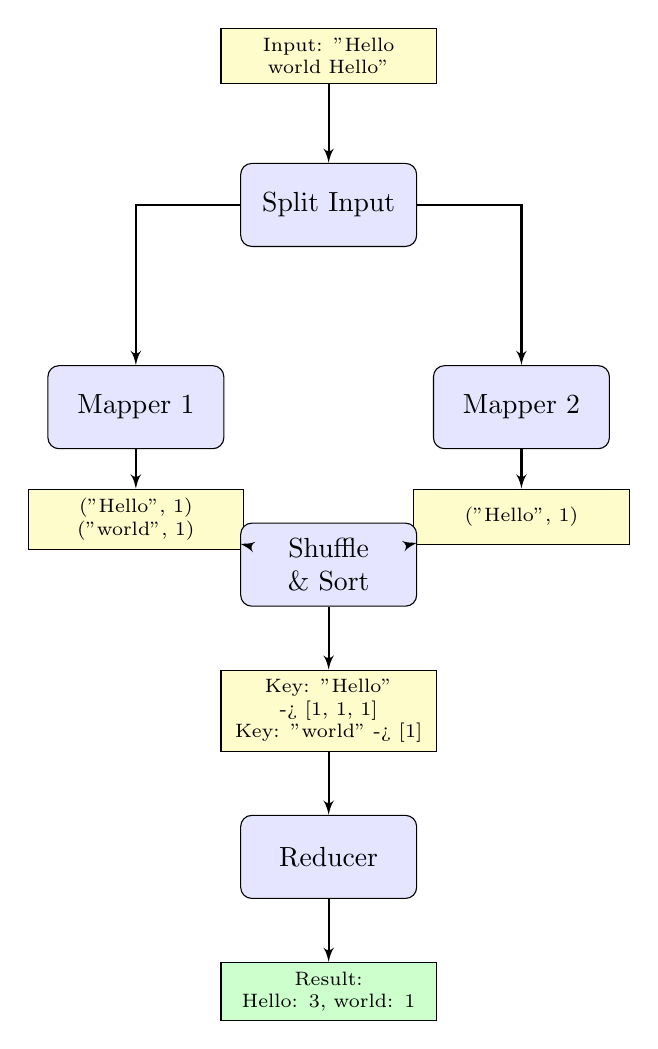
\begin{tikzpicture}[
        node distance=1.5cm and 1cm,
        process/.style={rectangle, draw, fill=blue!10, text width=2cm, text centered, rounded corners, minimum height=3em},
        data/.style={rectangle, draw, fill=yellow!20, text width=2.5cm, text centered, minimum height=2em, font=\scriptsize},
        line/.style={draw, -latex', thick}
    ]
    
    \node [data] (input) {Input: "Hello world Hello"};
    \node [process, below=1cm of input] (split) {Split Input};
    
    \node [process, below left=1.5cm and 0.2cm of split] (map1) {Mapper 1};
    \node [process, below right=1.5cm and 0.2cm of split] (map2) {Mapper 2};
    
    \node [data, below=0.5cm of map1] (out1) {("Hello", 1) ("world", 1)};
    \node [data, below=0.5cm of map2] (out2) {("Hello", 1)};
    
    \node [process, below=3.5cm of split] (shuffle) {Shuffle \& Sort};
    
    \node [data, below=0.8cm of shuffle] (group) {Key: "Hello" -> [1, 1, 1] \\ Key: "world" -> [1]};
    
    \node [process, below=0.8cm of group] (reduce) {Reducer};
    
    \node [data, below=0.8cm of reduce, fill=green!20] (final) {Result: \\ Hello: 3, world: 1};

    \path [line] (input) -- (split);
    \path [line] (split) -| (map1);
    \path [line] (split) -| (map2);
    \path [line] (map1) -- (out1);
    \path [line] (map2) -- (out2);
    \path [line] (out1) -- (shuffle);
    \path [line] (out2) -- (shuffle);
    \path [line] (shuffle) -- (group);
    \path [line] (group) -- (reduce);
    \path [line] (reduce) -- (final);
    
    \end{tikzpicture}
    \caption{MapReduce Data Flow for Word Count}
    \label{fig:wordcount_flow}
\end{figure}

\subsection{Mapper and Reducer Logic}

The \textbf{Mapper} takes a line of text, normalizes it (lowercase, remove punctuation), and emits a key-value pair \texttt{(word, 1)} for every word found.

\begin{lstlisting}[language=Python, caption=Mapper Implementation]
def mapper(self, text_chunk):
    output = []
    for line in text_chunk:
        words = clean_text(line).split()
        for word in words:
            output.append((word, 1))
    return output
\end{lstlisting}

The \textbf{Reducer} receives a key (word) and a list of counts (e.g., \texttt{[1, 1, 1]}). It sums these values to get the total frequency.

\begin{lstlisting}[language=Python, caption=Reducer Implementation]
def reducer(self, key, values):
    return (key, sum(values))
\end{lstlisting}

\section{Roles and Responsibilities}
\begin{table}[h]
\centering
\begin{tabular}{|c|l|l|}
\hline
\textbf{No.} & \textbf{Member} & \textbf{Task} \\ \hline
1 & Member 1 & Mapper logic and Input splitting \\ \hline
2 & Member 2 & Reducer logic and Shuffle implementation \\ \hline
3 & Member 3 & Report writing and Architecture Diagram \\ \hline
\end{tabular}
\caption{Group Roles}
\end{table}

\end{document}